\documentclass{standalone}
\usepackage{tikz}
\usetikzlibrary{patterns, positioning}

\begin{document}
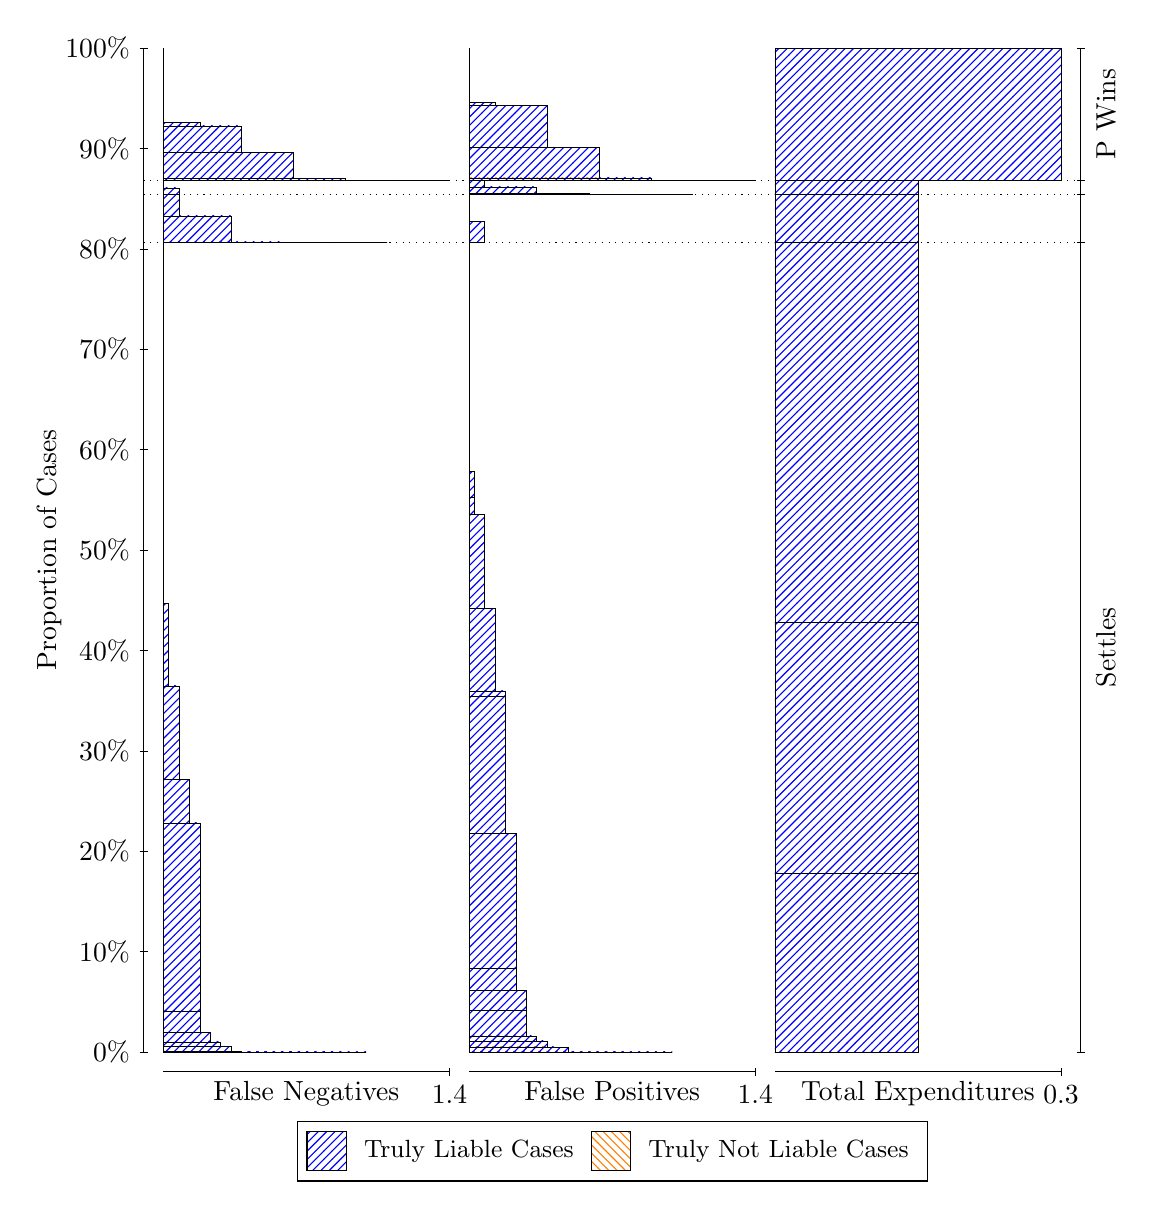
\begin{tikzpicture}
\draw[black, very thin] (1.5,1.75) -- (1.5,14.5);
\node[rotate=90, anchor=center] at (0.3, 8.125) {Proportion of Cases};
\draw[black, very thin] (1.45,1.75) -- (1.55,1.75);
\node[anchor=east] at (1.45, 1.75) {0\%};
\draw[black, very thin] (1.45,3.025) -- (1.55,3.025);
\node[anchor=east] at (1.45, 3.025) {10\%};
\draw[black, very thin] (1.45,4.3) -- (1.55,4.3);
\node[anchor=east] at (1.45, 4.3) {20\%};
\draw[black, very thin] (1.45,5.575) -- (1.55,5.575);
\node[anchor=east] at (1.45, 5.575) {30\%};
\draw[black, very thin] (1.45,6.85) -- (1.55,6.85);
\node[anchor=east] at (1.45, 6.85) {40\%};
\draw[black, very thin] (1.45,8.125) -- (1.55,8.125);
\node[anchor=east] at (1.45, 8.125) {50\%};
\draw[black, very thin] (1.45,9.4) -- (1.55,9.4);
\node[anchor=east] at (1.45, 9.4) {60\%};
\draw[black, very thin] (1.45,10.675) -- (1.55,10.675);
\node[anchor=east] at (1.45, 10.675) {70\%};
\draw[black, very thin] (1.45,11.95) -- (1.55,11.95);
\node[anchor=east] at (1.45, 11.95) {80\%};
\draw[black, very thin] (1.45,13.225) -- (1.55,13.225);
\node[anchor=east] at (1.45, 13.225) {90\%};
\draw[black, very thin] (1.45,14.5) -- (1.55,14.5);
\node[anchor=east] at (1.45, 14.5) {100\%};

\draw[black, very thin] (13.4,1.75) -- (13.4,14.5);
\draw[black, very thin] (13.35,1.75) -- (13.45,1.75);
\node[anchor=west] at (13.35, 1.75) {};
\draw[black, very thin] (13.35,12.031) -- (13.45,12.031);
\node[anchor=west] at (13.35, 12.031) {};
\draw[black, very thin] (13.35,12.64) -- (13.45,12.64);
\node[anchor=west] at (13.35, 12.64) {};
\draw[black, very thin] (13.35,12.822) -- (13.45,12.822);
\node[anchor=west] at (13.35, 12.822) {};
\draw[black, very thin] (13.35,14.5) -- (13.45,14.5);
\node[anchor=west] at (13.35, 14.5) {};

\draw[black, very thin, pattern color=blue, pattern=north east lines] (1.75,1.75) rectangle (4.3264,1.75);
\draw[black, very thin, pattern color=blue, pattern=north east lines] (1.75,1.75) rectangle (4.0621,1.75);
\draw[black, very thin, pattern color=blue, pattern=north east lines] (1.75,1.75) rectangle (3.7979,1.75);
\draw[black, very thin, pattern color=blue, pattern=north east lines] (1.75,1.75) rectangle (3.6658,1.75);
\draw[black, very thin, pattern color=blue, pattern=north east lines] (1.75,1.75) rectangle (3.5336,1.75);
\draw[black, very thin, pattern color=blue, pattern=north east lines] (1.75,1.75) rectangle (3.4015,1.75);
\draw[black, very thin, pattern color=blue, pattern=north east lines] (1.75,1.75) rectangle (3.2694,1.7501);
\draw[black, very thin, pattern color=blue, pattern=north east lines] (1.75,1.7501) rectangle (3.1373,1.7501);
\draw[black, very thin, pattern color=blue, pattern=north east lines] (1.75,1.7501) rectangle (3.0052,1.7503);
\draw[black, very thin, pattern color=blue, pattern=north east lines] (1.75,1.7503) rectangle (2.873,1.7503);
\draw[black, very thin, pattern color=blue, pattern=north east lines] (1.75,1.7503) rectangle (2.873,1.7509);
\draw[black, very thin, pattern color=blue, pattern=north east lines] (1.75,1.7509) rectangle (2.7409,1.7551);
\draw[black, very thin, pattern color=blue, pattern=north east lines] (1.75,1.7551) rectangle (2.6088,1.8227);
\draw[black, very thin, pattern color=blue, pattern=north east lines] (1.75,1.8227) rectangle (2.4767,1.8777);
\draw[black, very thin, pattern color=blue, pattern=north east lines] (1.75,1.8777) rectangle (2.3445,1.9967);
\draw[black, very thin, pattern color=blue, pattern=north east lines] (1.75,1.9967) rectangle (2.2124,1.9967);
\draw[black, very thin, pattern color=blue, pattern=north east lines] (1.75,1.9967) rectangle (2.2124,2.2713);
\draw[black, very thin, pattern color=blue, pattern=north east lines] (1.75,2.2713) rectangle (2.2124,4.6603);
\draw[black, very thin, pattern color=blue, pattern=north east lines] (1.75,4.6603) rectangle (2.0803,5.2072);
\draw[black, very thin, pattern color=blue, pattern=north east lines] (1.75,5.2072) rectangle (1.9482,6.4002);
\draw[black, very thin, pattern color=blue, pattern=north east lines] (1.75,6.4002) rectangle (1.8161,7.444);
\draw[black, very thin, pattern color=orange, pattern=north west lines] (1.75,7.444) rectangle (1.75,7.444);
\draw[black, very thin, pattern color=blue, pattern=north east lines] (1.75,7.444) rectangle (1.75,12.031);
\draw[black, very thin, pattern color=blue, pattern=north east lines] (1.75,12.031) rectangle (4.5906,12.031);
\draw[black, very thin, pattern color=blue, pattern=north east lines] (1.75,12.031) rectangle (3.93,12.031);
\draw[black, very thin, pattern color=blue, pattern=north east lines] (1.75,12.031) rectangle (3.2694,12.039);
\draw[black, very thin, pattern color=blue, pattern=north east lines] (1.75,12.039) rectangle (2.6088,12.368);
\draw[black, very thin, pattern color=blue, pattern=north east lines] (1.75,12.368) rectangle (1.9482,12.64);
\draw[black, very thin, pattern color=orange, pattern=north west lines] (1.75,12.64) rectangle (1.75,12.64);
\draw[black, very thin, pattern color=blue, pattern=north east lines] (1.75,12.64) rectangle (1.9482,12.725);
\draw[black, very thin, pattern color=orange, pattern=north west lines] (1.75,12.725) rectangle (1.75,12.725);
\draw[black, very thin, pattern color=blue, pattern=north east lines] (1.75,12.725) rectangle (1.75,12.822);
\draw[black, very thin, pattern color=blue, pattern=north east lines] (1.75,12.822) rectangle (5.3833,12.822);
\draw[black, very thin, pattern color=blue, pattern=north east lines] (1.75,12.822) rectangle (4.7227,12.822);
\draw[black, very thin, pattern color=blue, pattern=north east lines] (1.75,12.822) rectangle (4.0621,12.845);
\draw[black, very thin, pattern color=blue, pattern=north east lines] (1.75,12.845) rectangle (3.5336,12.845);
\draw[black, very thin, pattern color=blue, pattern=north east lines] (1.75,12.845) rectangle (3.4015,13.17);
\draw[black, very thin, pattern color=blue, pattern=north east lines] (1.75,13.17) rectangle (2.873,13.171);
\draw[black, very thin, pattern color=blue, pattern=north east lines] (1.75,13.171) rectangle (2.7409,13.512);
\draw[black, very thin, pattern color=blue, pattern=north east lines] (1.75,13.512) rectangle (2.2124,13.552);
\draw[black, very thin, pattern color=blue, pattern=north east lines] (1.75,13.552) rectangle (2.0803,13.553);
\draw[black, very thin, pattern color=orange, pattern=north west lines] (1.75,13.553) rectangle (1.75,13.553);
\draw[black, very thin, pattern color=blue, pattern=north east lines] (1.75,13.553) rectangle (1.75,14.5);
\draw[black, very thin, pattern color=orange, pattern=north west lines] (5.6333,1.75) rectangle (8.2097,1.75);
\draw[black, very thin, pattern color=blue, pattern=north east lines] (5.6333,1.75) rectangle (8.2097,1.75);
\draw[black, very thin, pattern color=orange, pattern=north west lines] (5.6333,1.75) rectangle (7.6812,1.75);
\draw[black, very thin, pattern color=blue, pattern=north east lines] (5.6333,1.75) rectangle (7.6812,1.75);
\draw[black, very thin, pattern color=blue, pattern=north east lines] (5.6333,1.75) rectangle (7.5491,1.75);
\draw[black, very thin, pattern color=orange, pattern=north west lines] (5.6333,1.75) rectangle (7.417,1.75);
\draw[black, very thin, pattern color=blue, pattern=north east lines] (5.6333,1.75) rectangle (7.417,1.75);
\draw[black, very thin, pattern color=orange, pattern=north west lines] (5.6333,1.75) rectangle (7.1527,1.75);
\draw[black, very thin, pattern color=blue, pattern=north east lines] (5.6333,1.75) rectangle (7.1527,1.75);
\draw[black, very thin, pattern color=blue, pattern=north east lines] (5.6333,1.75) rectangle (7.0206,1.7505);
\draw[black, very thin, pattern color=orange, pattern=north west lines] (5.6333,1.7505) rectangle (6.8885,1.7505);
\draw[black, very thin, pattern color=blue, pattern=north east lines] (5.6333,1.7505) rectangle (6.8885,1.7513);
\draw[black, very thin, pattern color=orange, pattern=north west lines] (5.6333,1.7513) rectangle (6.8885,1.7513);
\draw[black, very thin, pattern color=blue, pattern=north east lines] (5.6333,1.7513) rectangle (6.8885,1.8125);
\draw[black, very thin, pattern color=blue, pattern=north east lines] (5.6333,1.8125) rectangle (6.7564,1.8147);
\draw[black, very thin, pattern color=orange, pattern=north west lines] (5.6333,1.8147) rectangle (6.6242,1.8147);
\draw[black, very thin, pattern color=blue, pattern=north east lines] (5.6333,1.8147) rectangle (6.6242,1.8914);
\draw[black, very thin, pattern color=blue, pattern=north east lines] (5.6333,1.8914) rectangle (6.4921,1.9552);
\draw[black, very thin, pattern color=orange, pattern=north west lines] (5.6333,1.9552) rectangle (6.36,1.9552);
\draw[black, very thin, pattern color=blue, pattern=north east lines] (5.6333,1.9552) rectangle (6.36,2.2735);
\draw[black, very thin, pattern color=blue, pattern=north east lines] (5.6333,2.2735) rectangle (6.36,2.5367);
\draw[black, very thin, pattern color=blue, pattern=north east lines] (5.6333,2.5367) rectangle (6.2279,2.8113);
\draw[black, very thin, pattern color=blue, pattern=north east lines] (5.6333,2.8113) rectangle (6.2279,4.5252);
\draw[black, very thin, pattern color=orange, pattern=north west lines] (5.6333,4.5252) rectangle (6.0958,4.5252);
\draw[black, very thin, pattern color=blue, pattern=north east lines] (5.6333,4.5252) rectangle (6.0958,6.2727);
\draw[black, very thin, pattern color=blue, pattern=north east lines] (5.6333,6.2727) rectangle (6.0958,6.3366);
\draw[black, very thin, pattern color=blue, pattern=north east lines] (5.6333,6.3366) rectangle (5.9636,7.3804);
\draw[black, very thin, pattern color=blue, pattern=north east lines] (5.6333,7.3804) rectangle (5.8315,8.5735);
\draw[black, very thin, pattern color=blue, pattern=north east lines] (5.6333,8.5735) rectangle (5.6994,8.7994);
\draw[black, very thin, pattern color=blue, pattern=north east lines] (5.6333,8.7994) rectangle (5.6994,9.1204);
\draw[black, very thin, pattern color=blue, pattern=north east lines] (5.6333,9.1204) rectangle (5.6333,12.031);
\draw[black, very thin, pattern color=orange, pattern=north west lines] (5.6333,12.031) rectangle (5.8315,12.031);
\draw[black, very thin, pattern color=blue, pattern=north east lines] (5.6333,12.031) rectangle (5.8315,12.303);
\draw[black, very thin, pattern color=blue, pattern=north east lines] (5.6333,12.303) rectangle (5.6333,12.64);
\draw[black, very thin, pattern color=orange, pattern=north west lines] (5.6333,12.64) rectangle (8.4739,12.64);
\draw[black, very thin, pattern color=blue, pattern=north east lines] (5.6333,12.64) rectangle (8.4739,12.64);
\draw[black, very thin, pattern color=blue, pattern=north east lines] (5.6333,12.64) rectangle (7.8133,12.64);
\draw[black, very thin, pattern color=blue, pattern=north east lines] (5.6333,12.64) rectangle (7.1527,12.65);
\draw[black, very thin, pattern color=blue, pattern=north east lines] (5.6333,12.65) rectangle (6.4921,12.737);
\draw[black, very thin, pattern color=blue, pattern=north east lines] (5.6333,12.737) rectangle (5.8315,12.822);
\draw[black, very thin, pattern color=orange, pattern=north west lines] (5.6333,12.822) rectangle (9.2667,12.822);
\draw[black, very thin, pattern color=blue, pattern=north east lines] (5.6333,12.822) rectangle (9.2667,12.822);
\draw[black, very thin, pattern color=orange, pattern=north west lines] (5.6333,12.822) rectangle (8.6061,12.822);
\draw[black, very thin, pattern color=blue, pattern=north east lines] (5.6333,12.822) rectangle (8.6061,12.822);
\draw[black, very thin, pattern color=orange, pattern=north west lines] (5.6333,12.822) rectangle (7.9455,12.822);
\draw[black, very thin, pattern color=blue, pattern=north east lines] (5.6333,12.822) rectangle (7.9455,12.851);
\draw[black, very thin, pattern color=orange, pattern=north west lines] (5.6333,12.851) rectangle (7.2848,12.851);
\draw[black, very thin, pattern color=blue, pattern=north east lines] (5.6333,12.851) rectangle (7.2848,13.235);
\draw[black, very thin, pattern color=orange, pattern=north west lines] (5.6333,13.235) rectangle (6.7564,13.235);
\draw[black, very thin, pattern color=blue, pattern=north east lines] (5.6333,13.235) rectangle (6.7564,13.235);
\draw[black, very thin, pattern color=blue, pattern=north east lines] (5.6333,13.235) rectangle (6.6242,13.769);
\draw[black, very thin, pattern color=blue, pattern=north east lines] (5.6333,13.769) rectangle (6.0958,13.769);
\draw[black, very thin, pattern color=orange, pattern=north west lines] (5.6333,13.769) rectangle (6.0958,13.769);
\draw[black, very thin, pattern color=blue, pattern=north east lines] (5.6333,13.769) rectangle (6.0958,13.769);
\draw[black, very thin, pattern color=blue, pattern=north east lines] (5.6333,13.769) rectangle (5.9636,13.809);
\draw[black, very thin, pattern color=orange, pattern=north west lines] (5.6333,13.809) rectangle (5.6333,13.809);
\draw[black, very thin, pattern color=blue, pattern=north east lines] (5.6333,13.809) rectangle (5.6333,14.5);
\draw[black, very thin, pattern color=orange, pattern=north west lines] (9.5167,1.75) rectangle (11.333,1.75);
\draw[black, very thin, pattern color=blue, pattern=north east lines] (9.5167,1.75) rectangle (11.333,4.0207);
\draw[black, very thin, pattern color=orange, pattern=north west lines] (9.5167,4.0207) rectangle (11.333,4.0207);
\draw[black, very thin, pattern color=blue, pattern=north east lines] (9.5167,4.0207) rectangle (11.333,7.2048);
\draw[black, very thin, pattern color=orange, pattern=north west lines] (9.5167,7.2048) rectangle (11.333,7.2048);
\draw[black, very thin, pattern color=blue, pattern=north east lines] (9.5167,7.2048) rectangle (11.333,12.031);
\draw[black, very thin, pattern color=orange, pattern=north west lines] (9.5167,12.031) rectangle (11.333,12.031);
\draw[black, very thin, pattern color=blue, pattern=north east lines] (9.5167,12.031) rectangle (11.333,12.64);
\draw[black, very thin, pattern color=orange, pattern=north west lines] (9.5167,12.64) rectangle (11.333,12.64);
\draw[black, very thin, pattern color=blue, pattern=north east lines] (9.5167,12.64) rectangle (11.333,12.822);
\draw[black, very thin, pattern color=orange, pattern=north west lines] (9.5167,12.822) rectangle (13.15,12.822);
\draw[black, very thin, pattern color=blue, pattern=north east lines] (9.5167,12.822) rectangle (13.15,14.5);
\draw[black, dotted] (1.5,12.031) -- (13.4,12.031);
\draw[black, dotted] (1.5,12.64) -- (13.4,12.64);
\draw[black, dotted] (1.5,12.822) -- (13.4,12.822);
\draw[black, very thin] (1.75,1.5) -- (5.3833,1.5);
\node[anchor=north] at (3.5667, 1.5) {False Negatives};
\draw[black, very thin] (5.3833,1.45) -- (5.3833,1.55);
\node[anchor=north] at (5.3833, 1.45) {1.4};

\draw[black, very thin] (5.6333,1.5) -- (9.2667,1.5);
\node[anchor=north] at (7.45, 1.5) {False Positives};
\draw[black, very thin] (9.2667,1.45) -- (9.2667,1.55);
\node[anchor=north] at (9.2667, 1.45) {1.4};

\draw[black, very thin] (9.5167,1.5) -- (13.15,1.5);
\node[anchor=north] at (11.333, 1.5) {Total Expenditures};
\draw[black, very thin] (13.15,1.45) -- (13.15,1.55);
\node[anchor=north] at (13.15, 1.45) {0.3};

\node[black, centered, rotate=90] at (13.72, 6.8903) {Settles};


\node[black, centered, rotate=90] at (13.72, 13.661) {P Wins};

\draw (7.449999999999999,1.5) node[draw=none] (baseCoordinate) {};
\begin{scope}[align=center]
        \matrix[scale=0.5, draw=black, below=0.5cm of baseCoordinate, nodes={draw}, column sep=0.1cm]{
            \node[rectangle, draw, minimum width=0.5cm, minimum height=0.5cm, pattern=north east lines, pattern color=blue] {}; &
            \node[draw=none, font=\small] (B) {Truly Liable Cases}; &
            \node[rectangle, draw, minimum width=0.5cm, minimum height=0.5cm, pattern=north west lines, pattern color=orange] {}; &
            \node[draw=none, font=\small] (B) {Truly Not Liable Cases}; \\
            };
\end{scope}

\end{tikzpicture}
\end{document}